\section{Computing Clearance Value Annotations}
\label{aha:planningwithannotations}
On a grid map, a clearance value is perhaps best explained as representing the length or width of a square that begins at some octile being evaluated and is expanded symmetrically to the right and down until it intersects an obstacle.     
To make our ideas more concrete we will use as a running example a simple environment featuring two terrain types: Ground (represented as white tiles) and Trees (represented as grey tiles). 
To distinguish traversable tiles from non-traversable tiles we will colour hard obstacles black. 
The set of capabilities, $C$, required to traverse such a map is thus defined as $C = \lbrace \lbrace Ground \rbrace, \lbrace Trees \rbrace, \lbrace Ground \vee Trees \rbrace \rbrace$. 
We will work with agents of two sizes traversing across this environment and thus let $S = \lbrace 1, 2 \rbrace$.
\par \indent
Figure \ref{aha-fig:annotations} (a) to (d) illustrates how clearance can be computed with an iterative procedure in an environment as described above.
In Figure \ref{aha-fig:annotations}(a) the clearance square for the highlighted traversable target tile is initialised to 1. 
Subsequent iterations (Figures \ref{aha-fig:annotations}(b)-(c)) extend the square and increment the clearance. 
The process continues until the square contains an obstacle (Figure \ref{aha-fig:annotations}(d)) or extends beyond a map boundary at which point we terminate and do not increment clearance any further.
\par \indent
In Figure \ref{aha-fig:annotations}(e) we show the resultant clearance values for the single-terrain $\lbrace Ground \rbrace$ capability on a toy map example (note that we omit zero-value clearances).
Similarly, Figure \ref{aha-fig:annotations}(f) and Figure \ref{aha-fig:annotations}(g) show the clearance values associated with the $\lbrace Trees \rbrace$ and $\lbrace Ground \vee Trees \rbrace$ capabilities respectively.  

\begin{figure}[htbp]
	\vspace{-12pt}
       \caption{\emph{(a)-(d) Computing clearance. (e)-(g) Clearance values for different capabilities.}}
       \begin{center}
                       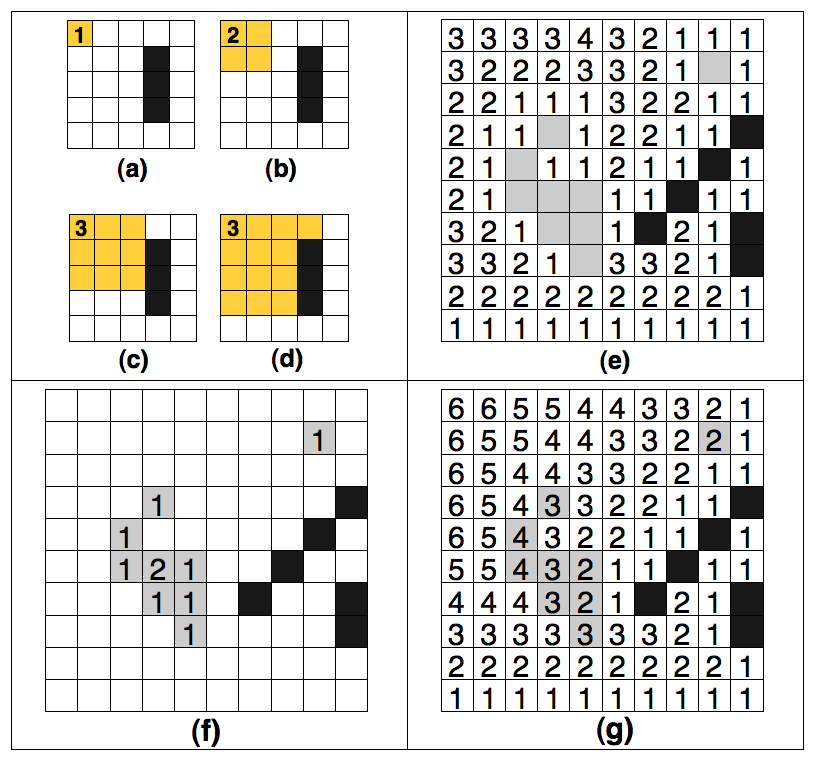
\includegraphics[scale=0.25, trim = 20mm 7mm 20mm 5mm]{diagrams/annotations.png}
       \end{center}
       \label{aha-fig:annotations}
	\vspace{-5pt}
\end{figure}

Once a clearance value is derived we store it in memory and repeat the entire procedure for each capability $c \in C$.  
The algorithm terminates when all octiles $t \in gridmap$ have been considered. 
The worst-case space complexity associated with computing clearance values in this fashion is thus characterised by: 
\begin{lemma}
\label{aha-lemma:numannotations}
Let $CV$ be the set of all clearance values required to annotate an octile gridmap with $r$ terrains. Further, let $G = (V, E)$ be a graph representing the gridmap where $V_{HO} \in V$ is the set of hard obstacles. Then, 
$$|CV| = (|V| - |V_{HO}|)\times \frac{2^{r-1}}{2}$$
\end{lemma}

\begin{proof}
For a node to be traversable for some capability, the capability must include the node's terrain type. 
There are $2^r$ capabilities but the maximum number of capabilities that include a node's terrain type is $\frac{2^{r-1}}{2}$. 
There are $|V|$ nodes in total to represent the envrionment, and we avoid storing any clearance values for all nodes in $V_{HO}$. 
\end{proof}

The result from Lemma \ref{aha-lemma:numannotations} is an upper bound; if no agent has a given capability $c$ there is no need to store the corresponding clearances.
Despite this observation, the associated exponential growth function suggests that it is impractical to store every clearance value as there are $\Theta(2^{r-1})$ per node.
Fortunately, clearance values can be computed on-demand with little effort. 
In particular, calculating clearance for any agent $a$ of size $s \in S$ only requires building a clearance square of maximum area $s^2$ octiles. 
We present such an approach in Algorithm \ref{aha-alg:calculateclearance}. 
\input algorithms/alg1_calculateclearance
\par \indent
The key advantage of calculating clearance is that we are able to plan for both large and small agents using a fixed size grid. 
We achieve this by mapping our extended problem into a classical problem with only two types of tiles (traversable and blocked) and reducing the problem to the case of a small-size agent that occupies the upper-left corner of the area required by the original, large-size agent. 
\begin{theorem}
\label{aha-theorem:reducibility}
Given an annotated grid map, any instance of a large-agent search problem can be reduced into a small-agent search problem, where the size of the small agent is one tile.
\end{theorem}

\begin{proof}
A tile $t$ is only traversable by an agent $a$ if $t$ has a clearance value $cv_{t}$ associated with the agent's capability $c_{a}$ which is at least as large as the size of the agent, $s_{a}$. 
\begin{equation}
\label{aha-equation:traversenode}
t(c_{a}) = cv_{t} \geq s_{a} : terrain(t) \in c_{a} \in C, s_{a} \in S
\end{equation}
If equation \ref{aha-equation:traversenode} holds, it must be the case that the terrain type of every tile in the clearance square used to compute $cv_{t}$ is included in $c_{a}$ and hence traversable for the agent. 
Thus, a large agent is able to navigate across a map by only considering the traversal requirements of the top-left node it will occupy.
\end{proof}
This is a useful result because it indicates that we can apply abstraction techniques from classical path planning to answer much more complex queries involving a wide range of terrain type and agent-size variables.
